\section{Before we Begin}\label{before-we-begin}

Our goals are lofty- introducing a new paradigm that combines data
mining with multi-objective optimization. And doing so in such a way
that even novices can understand, use, and adapt these tools for a large
range of new tasks.

But before we can start all that, we have to handle some preliminaries.
All artists, and programmers, should start out as apprentices. If we
were painters and this was Renaissance Italy, us apprentices would spend
decades study the ways of the masters, all the while preparing the
wooden panels for painting; agrinding and mixing pigments; drawing
preliminary sketches, copying paintings, and casting sculptures. It was
a good system that gave us the Michelangelo and Da Vinci who, in turn,
gave us the roof of the Sistine Chapel and the Mona Lisa.

In terms of this book, us apprentices first have to become effective
Python programmers. The rest of this chapter offers:

\begin{itemize}
\itemsep1pt\parskip0pt\parsep0pt
\item
  Some notes on useful web-based programming tools
\item
  Some pointers on learning Python
\item
  Some start-up exercises to test if you have an effective Python
  programming environment.
\end{itemize}

\subsection{Useful On-Line Tools}\label{useful-on-line-tools}

This book was written using the following on-line tools. There exists
many other great, readily available, tools (and if you know of better
ones, then please let me know (then maybe I'll switched over).

\subsubsection{Stackoverflow}\label{stackoverflow}

To find answers to nearly any question you'll ever want to ask about
Python, go browse:

\begin{lstlisting}
 http://stackoverflow.com/questions/tagged/python
\end{lstlisting}

\subsubsection{Cloud9}\label{cloud9}

If you do not want to install code locally on your machine, then there
are many readily-available on-line integrated development environments.

For example, to have root access to a fully-configured Unix
installation, you could go to

\begin{lstlisting}
 http://c9.io
\end{lstlisting}

One tip is to host your Cloud9 workspace files on Github. As of June
2015, the procedure for doing that was:

\begin{itemize}
\itemsep1pt\parskip0pt\parsep0pt
\item
  Go to Github and create an empty repository.
\item
  Log in to Cloud9 using your GitHub username (at \texttt{http://c9.io},
  there is a button for that, top right).
\item
  Hit the green \emph{CREATE NEW WORKSPACE} button

  \begin{itemize}
  \itemsep1pt\parskip0pt\parsep0pt
  \item
    Select \emph{Clone from URL};
  \item
    Find \emph{Source URL} and enter in
    \texttt{http://github.com/you/yourRepo}
  \item
    Wait ten seconds for the screen to change.
  \item
    Hit the green \emph{START EDITING} button.
  \end{itemize}
\end{itemize}

This will drop you into the wonderful Cloud9 integrated development
environment. Here, you can edit code and (using the above
\texttt{Makefile}) run \texttt{make\ typo} to backed up your code
outside Cloud9, over at \texttt{Github.com} (which means that if ever
Cloud9 goes away, you will still have your code).

The good news about Cloud9 is that it is very easy to setup and
configure. The bad news is that each Cloud9 workspace has the same
limits as Github- a 1GB size limit. Also, for CPU-intensive
applications, shared on-line resources like Cloud9 can be a little slow.
That said, for the newbie, Cloud9 is a very useful tool to jump start
the learning process.

For sites other than Cloud9, see Koding, Nitrous.IO and many more
besides.

\subsubsection{Github}\label{github}

All programmers should use off-site backup for their work. All
programmers working in teams should store their code in repositories
that let them fork a branch, work separately, then check back their
changes into the main trunk.

There are many freely-available repository tools. Github is one such
service that supports the \texttt{git} repository tool. Others include
SourceForge, BitBucket, and many more besides. Github has some special
advantages:

\begin{itemize}
\itemsep1pt\parskip0pt\parsep0pt
\item
  It is the center of vast social network of programmers;
\item
  Github support serving static web sites straight from your Github
  repo.
\item
  Many other services offer close integration with Github (e.g.~the
  Cloud9 tool discussed below).
\end{itemize}

For more information, go to:

\begin{lstlisting}
 http://github.com
\end{lstlisting}

The good news about Github is that it is very easy to setup and
configure. The bad news is that each Github repository has a 1GB size
limit. But that is certainly enough to get us started.

Regardless of whether or not you are using Github, you can use it to
access the source code used in this paper:

\begin{lstlisting}
# If you used "git":
git clone https://github.com/txt/evil
# If you just want the files:
wget https://github.com/txt/evil/archive/master.zip 
\end{lstlisting}

For Linux/Unix/Mac users, I add the following tip. In each of your
repository directories, add a \texttt{Makefile} with the following
contents.

\begin{lstlisting}
# File:  setup/Makefile (from github.com/txt/evil)
# Usage: make
typo:   ready
    @- git status
    @- git commit -am "saving"
    @- git push origin master # insert your branch names here

commit: ready
    @- git status
    @- git commit -a
    @- git push origin master

update: ready
    @- git pull origin master

status: ready
    @- git status

ready:
    @git config --global credential.helper cache
    @git config credential.helper 'cache --timeout=3600'

timm:  # <== change to your name
    @git config --global user.name "Tim Menzies" #<== your name
    @git config --global user.email tim.menzies@gmail.com #<== your email

tests: *ok.py
    @$(foreach f,$^,\
             printf "\n========= $f =========\n\n";\
             python $f;)
\end{lstlisting}

This \texttt{Makefile} implements some handy shortcuts:

\begin{itemize}
\itemsep1pt\parskip0pt\parsep0pt
\item
  \texttt{make\ typo} is a quick safety save-- do this many times per
  day;
\item
  \texttt{make\ commit} is for making commented commits-- use this to
  comment any improvements and/or degradation of functionality.
\item
  \texttt{make\ update} is for grabbing the latest version off the
  server-- do this at least at the start of each day.
\item
  \texttt{make\ status} is for finding files that are not currently
  known to Github.
\item
  \texttt{make\ ready} remembers your Github password for one hour-- use
  this if you use \texttt{make\ typo} a lot and you want to save some
  keystrokes.
\item
  \texttt{make\ timm} should be used if Github complains that it does
  not know who you are. Before running this one, edit this rule to
  include your name and email.
\item
  \texttt{make\ tests} is a little unit test engine, discussed later.
\end{itemize}

Tip:

\begin{itemize}
\itemsep1pt\parskip0pt\parsep0pt
\item
  IMPORTANT: When writing a \texttt{Makefile}, all indentations have to
  be made using the tab character, not 8 spaces.
\end{itemize}

Of course, there are 1000 other things you can do with a
\texttt{Makefile}. For example, this book is auto-generated by a
\texttt{Makefile} that automatically extracts comments and code from my
Python source code, then compiles the comments as Markdown, then used
the wonderful \texttt{pandoc} tool to compile the Markdown into Latex,
then converts the Latex to a \texttt{.pdf} file. Which is all
interesting stuff-- but beyond the scope of this book.

\subsection{Learning Python}\label{learning-python}

\subsubsection{Why Python?}\label{why-python}

I use Python for two reasons: readability and support. Like any computer
scientist, I yearn to use more powerful languages like LISP or
Javascript or Haskell (Have you tried them? They are \emph{great}
languages!). That said, it has to be said that good looking Python
\emph{reads} pretty good-- no ugly brackets, indentation standards
enforced by the compiler, simple keywords, etc.

Ah, you might reply, but what about other beautiful languages like
CoffeeScipt or Scala or insert yourFavoriteLanguageHere? It turns out
that, at the time of this writing, that there is more tutorial support
for Python that any other language I know. Apart from the many excellent
Python textbooks, the on-line community for Python is very active and
very helpful; e.g.~see stackoverlow.com.

\subsubsection{Which Python?}\label{which-python}

This book uses Python 2.7, rather than the latest-and-greatest version,
which is called Python3. Why?

The problems with Python3 are well-documented and being actively
addressed by the Python community. In short, many large and useful
Python libraries are not yet unavailable in Python3 so many developers
are sticking with the older version.

This situation may change in the near future so, in the coding standards
discussed below, we discuss how to use Python3 idioms while coding in
Python2. This will make our eventual jump to Python3 much easier.

\subsubsection{Installing}\label{installing}

To get going on Python, you will need a \emph{good} Python environment.
You may already have a favorite platform or interactive development
environment, in which case you can use that (and if not, you might
consider using the Cloud9 environment discussed above). To check if your
Python environment is \emph{good}, try changing and installing some
things.

Note that I use Mac/Linux/Unix so all the examples in this book will be
from a Unix-ish command-line prompt. For Windows users, you can

\begin{itemize}
\itemsep1pt\parskip0pt\parsep0pt
\item
  Use Google to find equivalent instructions for your platform;
\item
  Use some on-line IDE like Cloud9 (simple!).
\item
  Install a Linux in a virtual environment on top of Windows; e.g.~using
  VirtualBox and Ubuntu (warning: not so simple).
\end{itemize}

\paragraph{Code Indentation}\label{code-indentation}

Firstly, change the code indent to 2 spaces. Many editors have this
option. For example, for the editor I use (EMACS), those magic setting
can be found the \texttt{add-hock\ \textquotesingle{}python-model-hook}
of \texttt{.emacs} (available on-line at
\texttt{https://github.com/timm/timmnix} in the \texttt{dotemacs} file).

\paragraph{Get the Package Managers}\label{get-the-package-managers}

Secondly, make sure you have installed the \texttt{pip} and
\texttt{easy\_install} tools (these are tricks for quickly compiling
Python code). Try running

\begin{lstlisting}
pip -h
easy_install -h
\end{lstlisting}

Tips:

\begin{itemize}
\itemsep1pt\parskip0pt\parsep0pt
\item
  If these are not installed them Google for installation instructions.
  See also \texttt{https://pypi.python.org/pypi/setuptools} (which has
  hints for Windows users as well as those using Linix/Unix/Mac).
\item
  If you ever run this code and you get permission errors or some notice
  that you cannot update some directories, then run as superuser (by the
  way, one nice thing about Cloud9 is that you have superuser permission
  on your workspaces). To run code as superuser, in Linux/Unix/Mac,
  preface with \texttt{sudo}; e.g. \texttt{sudo\ pip} or
  \texttt{sudo\ pip\_install}
\end{itemize}

\paragraph{Use the Package Managers}\label{use-the-package-managers}

Thirdly, do some installs of various packages. Note that we will make
extensive use of all of the following.

\textbf{Package1: watcher.} Enable a \emph{watcher} on files that are
being edited. Every time you save the \emph{watched} file, it is
re-executed (so you get rapid feedback on your progress):

\begin{lstlisting}
sudo pip install rerun
\end{lstlisting}

Example: establish a \emph{watch} on \texttt{lib.py}:

\begin{lstlisting}
rerun "python lib.py"
\end{lstlisting}

Now, if ever we change any files in this directory, then this code will
rerun \texttt{python\ lib.py}-- which is a nice trick for getting very
fast feedback on code.

\textbf{Package2: 2D plotting with \texttt{matplotlib}.}

Run this code.

\begin{lstlisting}
sudo pip install matplotlib
\end{lstlisting}

Example: The following code, shows how to generate a plot within Cloud9
using \texttt{matplotlib}. To check if you have have a \emph{good}
Python environment, check you can run this code using
\texttt{python\ demoMatplot.py}. If you do not know Python yet, do not
try to understand the code (just download it and run it).

\newpage

\begin{lstlisting}
# File : setup/demoMatplot.py (from github.com/evil)
# Usage: python demoMatplot.py              
#                                           TRICKS
import matplotlib
matplotlib.use('Agg')     #.................... 1
import matplotlib.pyplot as plt 

def lines(xlabel, ylabel, title,
          f="lines.png",   #................... 2
          xsize=5,ysize=5,lines=[]): 
  width = len(lines[0][1:])
  xs = [x for x in xrange(1,width+1)] 
  plt.figure(figsize=(xsize,ysize))  #......... 3
  plt.xlabel(xlabel)
  plt.ylabel(ylabel) 
  for line in lines: 
    plt.plot(xs,  line[1:],  #................. 4a
                 label = line[0])   #.......... 4b
   
  plt.locator_params(nbins=len(xs)) #.......... 5
  plt.title(title)
  plt.legend()
  plt.tight_layout()                #.......... 6
  plt.savefig(f)

lines("days","production",  #.................. 7
      "Fruit output",
      xsize=3,ysize=3,lines=[
      ["apples",4,3,2,1],
      ["oranges",9,4,1,0.5]])
\end{lstlisting}

If the code works you should see the following file \texttt{lines.out}:

\begin{figure}[htbp]
\centering
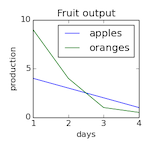
\includegraphics{img/matplotlib101.png}
\caption{Example, 2d plotting from Python, using \texttt{matplotlib}}
\end{figure}

If you do know Python, they I add notes on seven little tricks in the
above code:

\begin{enumerate}
\def\labelenumi{\arabic{enumi}.}
\itemsep1pt\parskip0pt\parsep0pt
\item
  Add this line \emph{right after} importing \texttt{matplotlib}. If
  absent, then when used in a non-X-server environment (e.g.~Cloud9),
  the code crashes.
\item
  Note the use of default parameters. By default, this function writes
  to \texttt{lines.png} but this can be changed when the function is
  called.
\item
  Here we can change the default size of a plot (which defaults to five
  inches square-- do you know why? hint: look at the default parameters
  of the function).
\item
  The line label and the line data is pulled from the data passed to the
  function. To see that, have a look at the last like of the code where
  \texttt{orange} is the first item in the list and the rest is data.
\item
  This is a hack to stop \texttt{matplotlib} adding in ticks like
  ``1.5''. With this hack, the number of ticks is equal to the number of
  items in each line to be plotted.
\item
  Another hack. Once we resize a plot, sometimes the label text gets cut
  off. The fix is to use a \texttt{tight\textbackslash{}\_layout}.
\item
  A sample call to this function.
\end{enumerate}

\textbf{Package3: some data miners.} If you've got \texttt{matplotlib}
working, then the next test is to install a more complex package like
\texttt{scikit-learn}. This is a nice collection of very useful data
mining tools. The following code will install \texttt{scikit-learn} on
Cloud9 (and for install instructions for other platforms, Google
\emph{sklearn}). If you do not know bash scripting, don't try to
understand the code, just run it using \texttt{bash\ sk.sh}.

\begin{lstlisting}
# File    : setup/sk.sh (from github.com/txt/evil)
# Usage   : bash sk.sh
installingBuildDependencies() {
  sudo apt-get install \
    build-essential python-dev python-setuptools \
    python-numpy python-scipy \
    libatlas-dev libatlas3gf-base
}
BLASandLAPACK() { 
 sudo update-alternatives --set libblas.so.3 \
    /usr/lib/atlas-base/atlas/libblas.so.3
 sudo update-alternatives --set liblapack.so.3 \
    /usr/lib/atlas-base/atlas/liblapack.so.3
}
matplotlib() { # just incase you have not done matplotlib yet
  sudo apt-get install python-matplotlib
}
sklearn() {
  pip install --user  --install-option="--prefix=" -U scikit-learn
}
installingBuildDependencies
BLASandLAPACK
matplotlib
sklearn
\end{lstlisting}

To check if this all works, then run the following code and look for a
generated image file called \texttt{sk.png}. Once again, if you do not
know Python yet, don't try to understand this code; just run it using
\texttt{python\ sk.py}

\begin{lstlisting}
# File:  setup/sk.py (from github.com/txt/evil)
# Usage: python sk.py
from sklearn import datasets
from sklearn.cross_validation import cross_val_predict
from sklearn import linear_model
import matplotlib
matplotlib.use('Agg')
import matplotlib.pyplot as plt

lr = linear_model.LinearRegression()
boston = datasets.load_boston()
y = boston.target
predicted = cross_val_predict(lr, boston.data, y, cv=10)
fig,ax = plt.subplots()
ax.scatter(y, predicted)
ax.plot([y.min(), y.max()], [y.min(), y.max()], 'k--', lw=4)
ax.set_xlabel('Measured')
ax.set_ylabel('Predicted')
fig.savefig('sk.png')
\end{lstlisting}

If that works, then the file \texttt{sk.png} should look like this:

\begin{figure}[htbp]
\centering
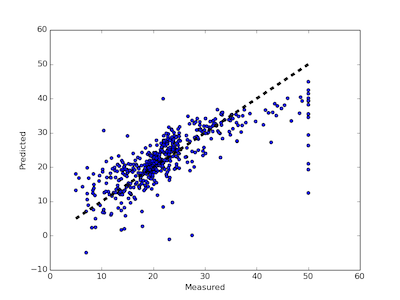
\includegraphics{img/sk.png}
\caption{Predictions generated by a machine learner.}
\end{figure}

\subsubsection{Python 101}\label{python-101}

There are many great tools for learning Python, including all the
on-line tools listed above.

In terms of a textbook, I highly recommend \emph{How to Think Like a
Computer Scientist} by Allen Downey, which can be purchased as a paper
book or viewed or downloaded from
\texttt{www.greenteapress.com/thinkpython}. All the source code from
that book is available on-line at:

\begin{lstlisting}
 https://github.com/AllenDowney/ThinkPython
\end{lstlisting}

If you liked that book, it would be good manners to make a small
donation to Prof.~Downey at that website-- but that is entirely up to
you.

Note that there are Python3 versions of this code, available on the web.
Try to avoid those.

In terms of a three week teach yourself program, I recommend the
following.

\begin{itemize}
\itemsep1pt\parskip0pt\parsep0pt
\item
  \textbf{Week1} Read chapters one to four. \emph{Do} exercises
  3.1,3.2,3.3,3.4,3.5. \emph{Do} install \texttt{Swampy} \emph{Do}
  exercise 4.2,4.3 (but makeIn terms of a three-week teach-= yoAt the
  time of this writing, at
\end{itemize}

tutorial mater

\subsubsection{Installing a ``Good'' Python
Environment}\label{installing-a-good-python-environment}

\subsubsection{Python Standards}\label{python-standards}

This textbook uses Python 2.7 for its code base. Of course, it is
tempting to use Python3 but there are still too many Python packages out
there t

\subsection{Mantras}\label{mantras}

\subsubsection{\texorpdfstring{``Do go coding, go for
feedback''}{Do go coding, go for feedback}}\label{do-go-coding-go-for-feedback}

\subsubsection{\texorpdfstring{``Red, Green,
Refactor''}{Red, Green, Refactor}}\label{red-green-refactor}

\subsubsection{\texorpdfstring{``Write Less
Code''}{Write Less Code}}\label{write-less-code}

Holzmann. true

\subsubsection{\texorpdfstring{``Stop writing
classes''}{Stop writing classes}}\label{stop-writing-classes}

Jack Diederich

\subsubsection{\texorpdfstring{``That needs a
DSL''}{That needs a DSL}}\label{that-needs-a-dsl}

Domain specific languages

\subsection{Homework}\label{homework}

\subsubsection{Homework1}\label{homework1}

\begin{itemize}
\item
  Do: get an account at \texttt{http://github.com}. Hand-in: your Github
  id.
\item
  Show that you have a \emph{good} Python environment by installing
\item
  Generate some pretty print python (2 space indent)
\end{itemize}
